\documentclass[11pt]{article}

\usepackage[margin=1.1in]{geometry}
\usepackage{amsmath, amssymb}
\usepackage{graphicx}
\usepackage{xcolor}
\usepackage[colorlinks=true, linkcolor=black, urlcolor=blue]{hyperref}
\usepackage{parskip}
\usepackage{enumitem}
\usepackage{mdframed}
\usepackage{booktabs}

\definecolor{boxbg}{HTML}{F4F6FA}
\definecolor{rule}{HTML}{C9D2E3}
\definecolor{accent}{HTML}{EA580C}

\newmdenv[backgroundcolor=boxbg, linecolor=rule, linewidth=0.7pt,
          innertopmargin=8pt, innerbottommargin=8pt,
          innerleftmargin=11pt, innerrightmargin=11pt,
          skipabove=10pt, skipbelow=10pt]{keybox}

\newcommand{\hl}[1]{\textcolor{accent}{\textbf{#1}}}
\newcommand{\means}{\textbf{\textcolor{accent}{What this means.}}\ }

\title{\bfseries Testing ECLIPSE Against 12 Other Ways of Drawing the Map\\[5pt]
\large What I found}
\author{Timothy Hsu \\ \small Aresty Summer Science Research Program}
\date{}

\begin{document}
\maketitle

\section*{What ECLIPSE is}

\textbf{ECLIPSE} --- \emph{Eigen-Combined Lens Integrating Predictions, Spread, and
Ensembles}. The name came first and the expansion was fitted to it afterwards, but each
word is doing real work: \emph{Predictions} is what the model is deciding, \emph{Spread}
is how people differ from one another, and \emph{Ensembles} is the crowd of other models
that fit the data just as well. ECLIPSE combines all three into one flat picture.

It exists because of a problem in the tool it was built for, GLIMPSE. A person is a list
of twenty or fifty numbers. To show someone where they stand, all of that has to be
squashed onto a flat page. The standard way of squashing, PCA, arranges people only by
how they differ from each other in general --- it knows nothing about what the model is
actually deciding. ECLIPSE is an attempt to squash people onto a page \emph{while keeping
the decision visible}.

This report is the test of whether that worked.

\section*{What I tested}

Thirteen methods of flattening data onto a page --- PCA, Random, LDA, PLS, NCA,
KernelPCA, Isomap, t-SNE, UMAP, PaCMAP, two kinds of neural-network autoencoder, and
ECLIPSE --- across seven real datasets: diabetes screening, credit risk, breast cancer
diagnosis, German and Taiwanese loan data, heart disease, and spam. Nearly
\hl{30,000 people} in total.

Each method was built using only half of each dataset, then scored on the half it had
never seen. That matters: the tool's whole point is that a new person types in their own
numbers and gets placed on a map that was built without them.

\begin{keybox}
\textbf{The four things I measured, in plain words.}
\begin{itemize}[leftmargin=*, itemsep=2pt, topsep=3pt]
  \item \textbf{Can you read the verdict off the picture?} If you only saw the map, could
        you tell what the model decided about someone from where their dot sits?
  \item \textbf{Are the two groups visibly apart?} Do the ``yes'' people and the ``no''
        people end up in different places, or smeared together?
  \item \textbf{Can a spot be turned back into a person?} Point at somewhere on the map
        --- can the tool tell you what real human being belongs there?
  \item \textbf{Are neighbours on screen real neighbours?} If two dots look close, are
        those two people actually similar?
\end{itemize}
\end{keybox}

\section*{What I found}

\subsection*{1. ECLIPSE beat all twelve at showing what the model decided}

ECLIPSE scored \hl{0.982}. PCA scored 0.849, the supervised autoencoder 0.865, t-SNE
0.812, UMAP 0.790, and a deliberately useless random baseline 0.565. ECLIPSE was the
single best method on 3 of the 7 datasets and close behind on the rest.

\means On an ECLIPSE map, \emph{where you are tells you what the model thinks of you}.
On a PCA map it only roughly does. Picture two dots sitting right next to each other.
On the PCA map, one of those people can be at 20\% risk and the other at 70\% --- they
look like similar cases and they are not. On the ECLIPSE map, close together really does
mean similar risk. The picture stops lying to the person reading it.

\begin{center}
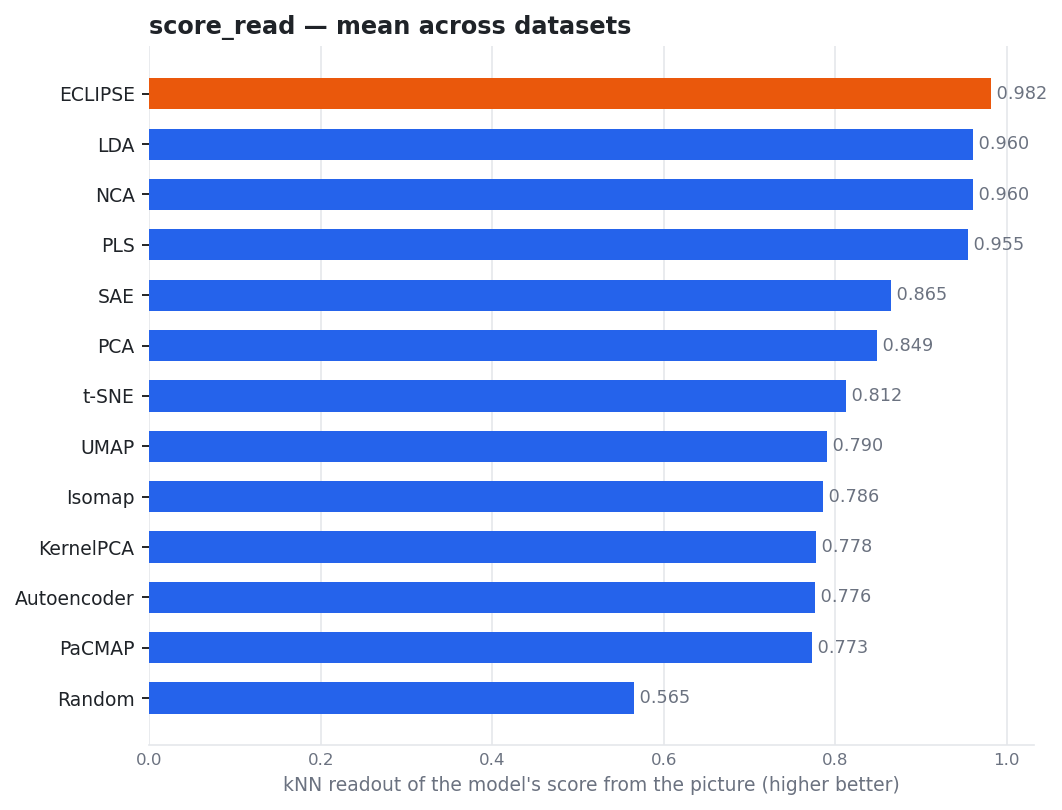
\includegraphics[width=0.80\textwidth]{figures/bars_score_read.png}
\end{center}

\subsection*{2. ECLIPSE beat all twelve at keeping the two groups apart}

ECLIPSE scored \hl{0.847}, just ahead of LDA and NCA (both 0.843), then PCA at 0.813 and
PaCMAP at 0.753.

\means The people who got a ``yes'' and the people who got a ``no'' land in visibly
different parts of the picture instead of being mixed together in one cloud. A patient
looking at the screen can see which side of the line they are on, and roughly how far
from it they are --- which is the first thing anybody wants to know.

\subsection*{3. ECLIPSE beat all the others at turning a spot back into a person}

This was the biggest margin in the whole study. ECLIPSE scored \hl{0.997} and was the
best method on \hl{6 of the 7 datasets}. PCA managed 0.865, the autoencoder 0.812,
KernelPCA 0.799, UMAP 0.715.

\means This is what makes advice possible. The tool tells someone: \emph{``if your
glucose were 118 instead of 142, the decision would flip.''} To say that, it has to take
a spot on the map and translate it back into real numbers in real units. ECLIPSE's
translation is almost perfect. KernelPCA's, at 0.799, is unreliable --- it would hand
someone a target that does not actually correspond to the spot on the screen, and they
would do the work and still be refused. A near-perfect score here is the difference
between advice you can act on and advice that quietly misleads.

\subsection*{4. Across everything, ECLIPSE came first}

Averaging the rankings across all four measures and all seven datasets, ECLIPSE placed
\hl{first of thirteen} (average rank 5.02), ahead of NCA (5.54), t-SNE (5.61), PLS
(5.93), LDA (6.04) and PCA (6.46). Random came last at 11.52.

\means No other method was better balanced. Several methods beat ECLIPSE on one measure
and then fell apart on another. ECLIPSE was the only one that was near the top on
everything that matters at once.

\subsection*{5. Three of the thirteen could not be used at all --- including the one
with the best score}

This surprised me most. \hl{t-SNE had the best neighbour-faithfulness score in the entire
study} --- 0.900, the best method on all seven datasets --- and it cannot be used for
this tool under any circumstances. Isomap and PaCMAP also had to be ruled out.

\means t-SNE can only draw the people it has already seen. A new patient walks in, types
in their numbers, and t-SNE simply has no answer for where to put them --- the whole
interaction the tool is built around is impossible. Isomap and PaCMAP can place a new
person, but they cannot run backwards, so they can never answer ``what would I have to
change?''. Only \hl{10 of the 13} methods are usable here at all.

In the figure below --- the same 768 people drawn by every method --- the t-SNE panel is
simply empty, with the words \emph{cannot place new people} in it. That blank square is
one of the findings.

\begin{center}
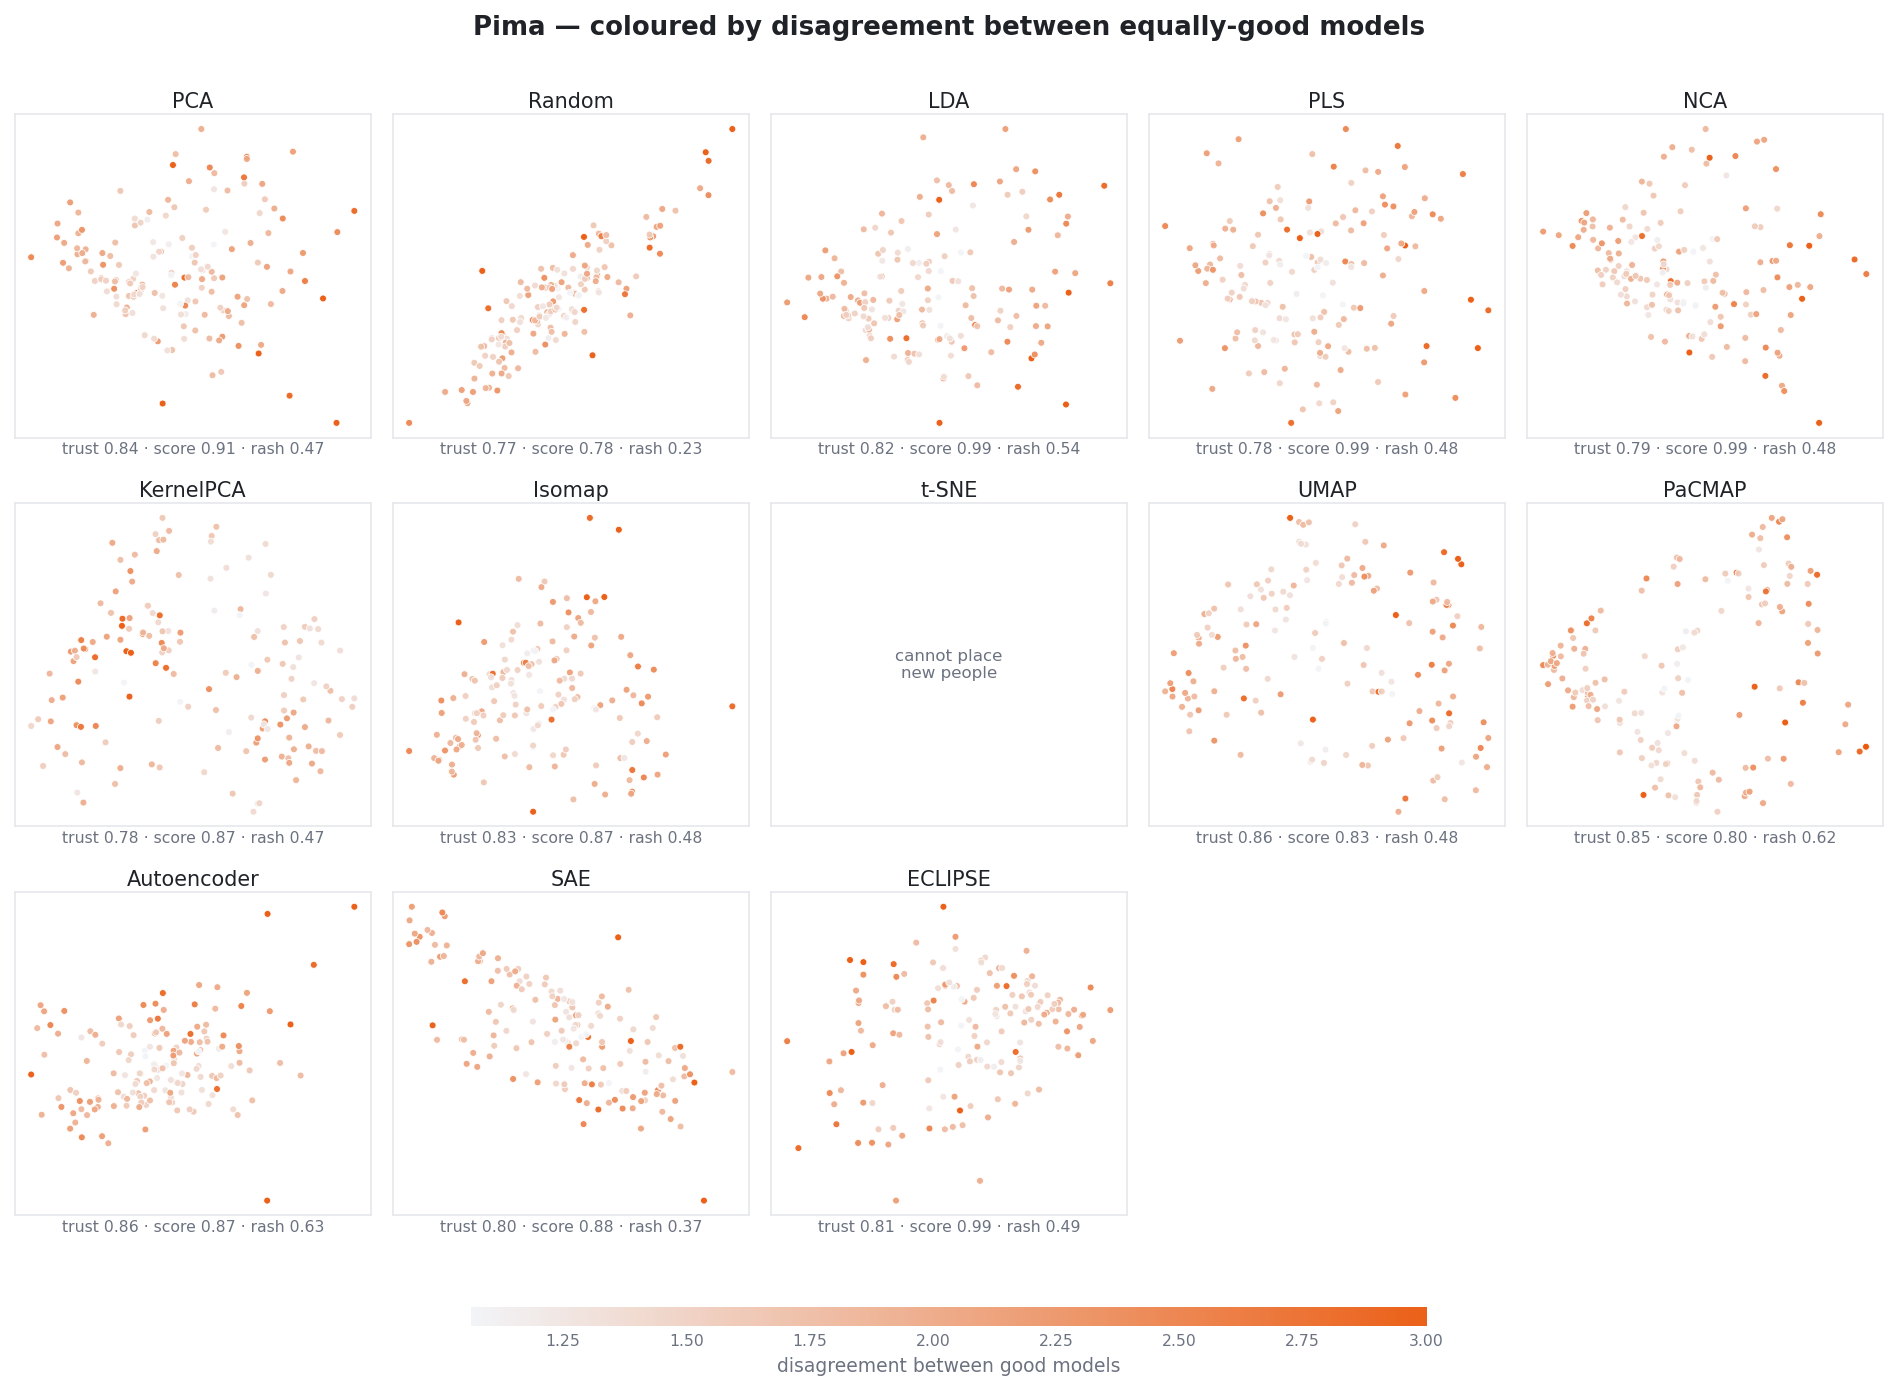
\includegraphics[width=\textwidth]{figures/grid_pima_rash.png}
\end{center}

\section*{Where ECLIPSE did worse}

\subsection*{It is only 7th of 13 at keeping neighbours honest}

ECLIPSE scored 0.763 here, behind t-SNE (0.900), UMAP (0.850), PaCMAP (0.843) and PCA
(0.787).

\means Two dots that look close together on an ECLIPSE map are slightly less likely to be
genuinely similar people than they would be on a PCA map. This is a deliberate trade, not
a flaw --- the method is allowed to give up a small amount of this in order to buy a much
larger gain elsewhere. It spent 0.024 of neighbour-honesty and bought 0.133 of
verdict-readability. That is a good trade, but it is a real cost and worth stating.

\subsection*{The disagreement result is not yet solid}

This is the honest weak point. The whole reason ECLIPSE exists is to show
\emph{disagreement between equally good models}, and on that specific measure ECLIPSE
beat PCA on only \hl{4 of the 7 datasets}, by an average of $+0.018$. Take away the one
dataset where it does exceptionally well (spam) and the average gain turns slightly
\emph{negative}. A different method, KernelPCA, scored much better here (0.708 against
ECLIPSE's 0.539).

\means ECLIPSE is proven as the best \emph{readable decision map}. It is \emph{not yet}
proven as a disagreement map, which is the thing it was named for. Two caveats soften
this. KernelPCA cannot actually be used --- it is the same method whose spot-to-person
translation scored 0.799, so its picture ranks disagreement well while its advice would
be wrong. And this measure is noisy on seven datasets. But the honest statement today is
that this part needs more testing, not that it has been won.

\section*{Bottom line}

\begin{keybox}
Against twelve alternatives on seven datasets and nearly 30,000 people, ECLIPSE came
\hl{first overall}, and won outright on the three things the tool depends on most: you
can read the model's verdict off the picture, the two outcome groups stay visibly apart,
and a spot on the map can be turned back into a real person with real numbers. It gives
up a small, deliberate amount of neighbour-faithfulness to get there.

The open question is the one it is named for. Showing \emph{disagreement between equally
good models} is where the evidence is thinnest --- a win on 4 of 7 datasets, driven
largely by one. That is the next thing to test properly.
\end{keybox}

\vfill
\noindent\footnotesize
\textit{Every number here comes from \texttt{alternative\_projection\_testing.ipynb} and
can be reproduced from \texttt{results/benchmark\_raw.csv}. The method itself is
explained in \texttt{glimpse\_and\_eclipse\_explained.tex}.}

\end{document}
